\documentclass[12pt]{extarticle}
\usepackage{amsmath, amsthm, amssymb, color}
\usepackage[colorlinks=true,linkcolor=blue,urlcolor=blue]{hyperref}
\usepackage{graphicx}
\usepackage{caption}
\usepackage{mathtools}
\usepackage{enumitem}
% \usepackage[all]{xypic}
\usepackage{verbatim}
\usepackage{tikz}
\usetikzlibrary{matrix}
\usetikzlibrary{arrows}
% \usepackage[linesnumbered,lined,commentsnumbered,ruled]{algorithm2e}
\usepackage{algorithm}
\usepackage[noend]{algpseudocode}
\usepackage{caption}
\usepackage[normalem]{ulem}
\usepackage{subcaption}
\tolerance 10000
\headheight 0in
\headsep 0in
\evensidemargin 0in
\oddsidemargin \evensidemargin
\textwidth 6.5in
\topmargin .25in
\textheight 8.8in

\synctex=1
\usepackage{makecell}
\usepackage{array}

% \theoremstyle{theorem}
\newtheorem{theorem}{Theorem}
\newtheorem{proposition}[theorem]{Proposition}
\newtheorem{lemma}[theorem]{Lemma}
\newtheorem{corollary}[theorem]{Corollary}
\newtheorem{algo}[theorem]{Algorithm}
\theoremstyle{definition}
\newtheorem{definition}[theorem]{Definition}
\newtheorem{problem}[theorem]{Problem}
\newtheorem{remark}[theorem]{Remark}
\newtheorem{conjecture}[theorem]{Conjecture}
\newtheorem{cor}[theorem]{Corollary}
\newtheorem{example}[theorem]{Example}
\newtheorem{exercise}[theorem]{Exercise}
\newtheorem{notation}[theorem]{Notation}
\newtheorem{fct}[theorem]{Fact}
\newtheorem{question}[theorem]{Question}
\numberwithin{theorem}{section}

\newcommand{\PP}{\mathbb{P}}
\newcommand{\RR}{\mathbb{R}}
\newcommand{\QQ}{\mathbb{Q}}
\newcommand{\CC}{\mathbb{C} }
\newcommand{\ZZ}{\mathbb{Z}}
\newcommand{\FF}{\mathbb{F}}
\newcommand{\NN}{\mathbb{N}}
\newcommand{\KK}{\mathbb{K}}

\newcommand{\defas}{\coloneqq}

\usepackage{stmaryrd}
\newcommand{\A}{\mathcal{A}}
\newcommand{\CIR}[1]{\llbracket#1\rrbracket}
\newcommand{\Set}[1]{\{#1\}}
\newcommand{\CI}{\mathbin{\perp \!\! \perp}}
\newcommand{\tri}{\triangle}

\title{\bf  CI Models from Graphs and Matroids}
\author{Tobias Boege, Sonja Petrovi\'c and Bernd Sturmfels}

\date{}

\begin{document}
\maketitle




\section*{The basis of the zero-margin part of the model from Ho\c{s}ten-Sullivant} 

\cite[Theorem 2.6]{HoSu02} provides the dimension formula for the space of tables all of whose $\Delta$ margins are zero. (That is, for the kernel of the toric map parametrizing the model of $\Delta$-independence.) %   the one with marginal independence for all faces of $\Delta$. 
Since the model is toric, the proof amounts to simply computing the vector space dimension of the kernel of the linear map induced by $\Delta$ by identifying the appropriate number of linearly independent vectors, which comprise the basis of the vectors space of tensors whose $\Delta$-margins are all zero.  Ho\c{s}ten and Sullivant identify  the basis as the exponents of adjacent minors as follows.

Let $S\not\in\Delta$ be a non-face of the complex. An adjacent minor $X$ supported on $S$ is defined as: 
\[
	X_{k_1\dots k_n} =(-1)^{\sum_{j\in S}\epsilon_j}, 
\]
where $k_j=i_j+\epsilon_j$, $\epsilon_j\in\{0,1\}$ and $j\in S$, and $k_j=0$ otherwise.

Let us see some small examples. 
For a $2\times\dots\times2$ tensor, for example if $S=\{12\}$, this amounts to the following set of  $2\times 2$ minors
% supported on the indices in the non-face $S$, and 
 located at the  first slice along all indices in the complement of $S$: 
\begin{align*}
	X_{000\dots0} = +1, \qquad X_{010\dots0} =-1,\\ 
	X_{100\dots0} =-1, \qquad 	X_{110\dots0}  =+1.
\end{align*}
Similarly, an adjacent minor supported on $S=\{123\}$ then we get the $2\times2\times2$ minor: 
\begin{align*}
	X_{0000\dots0} = +1, \qquad X_{0010\dots0} =-1,\\ 
	X_{0100\dots0} = -1, \qquad X_{0110\dots0} =+1,\\ 
	X_{1000\dots0} = -1, \qquad X_{1010\dots0} =+1,\\ 	
	X_{1100\dots0} =+1, \qquad 	X_{1110\dots0}  =-1.
\end{align*}

In \cite[Example 2.4]{HoSu02}, where $n=3$ and $S=\{2,3\}$, all nonzero entries ($\pm 1$) of the minors occur in the $i=0$ slice, which are the green shaded cells in this picture: 

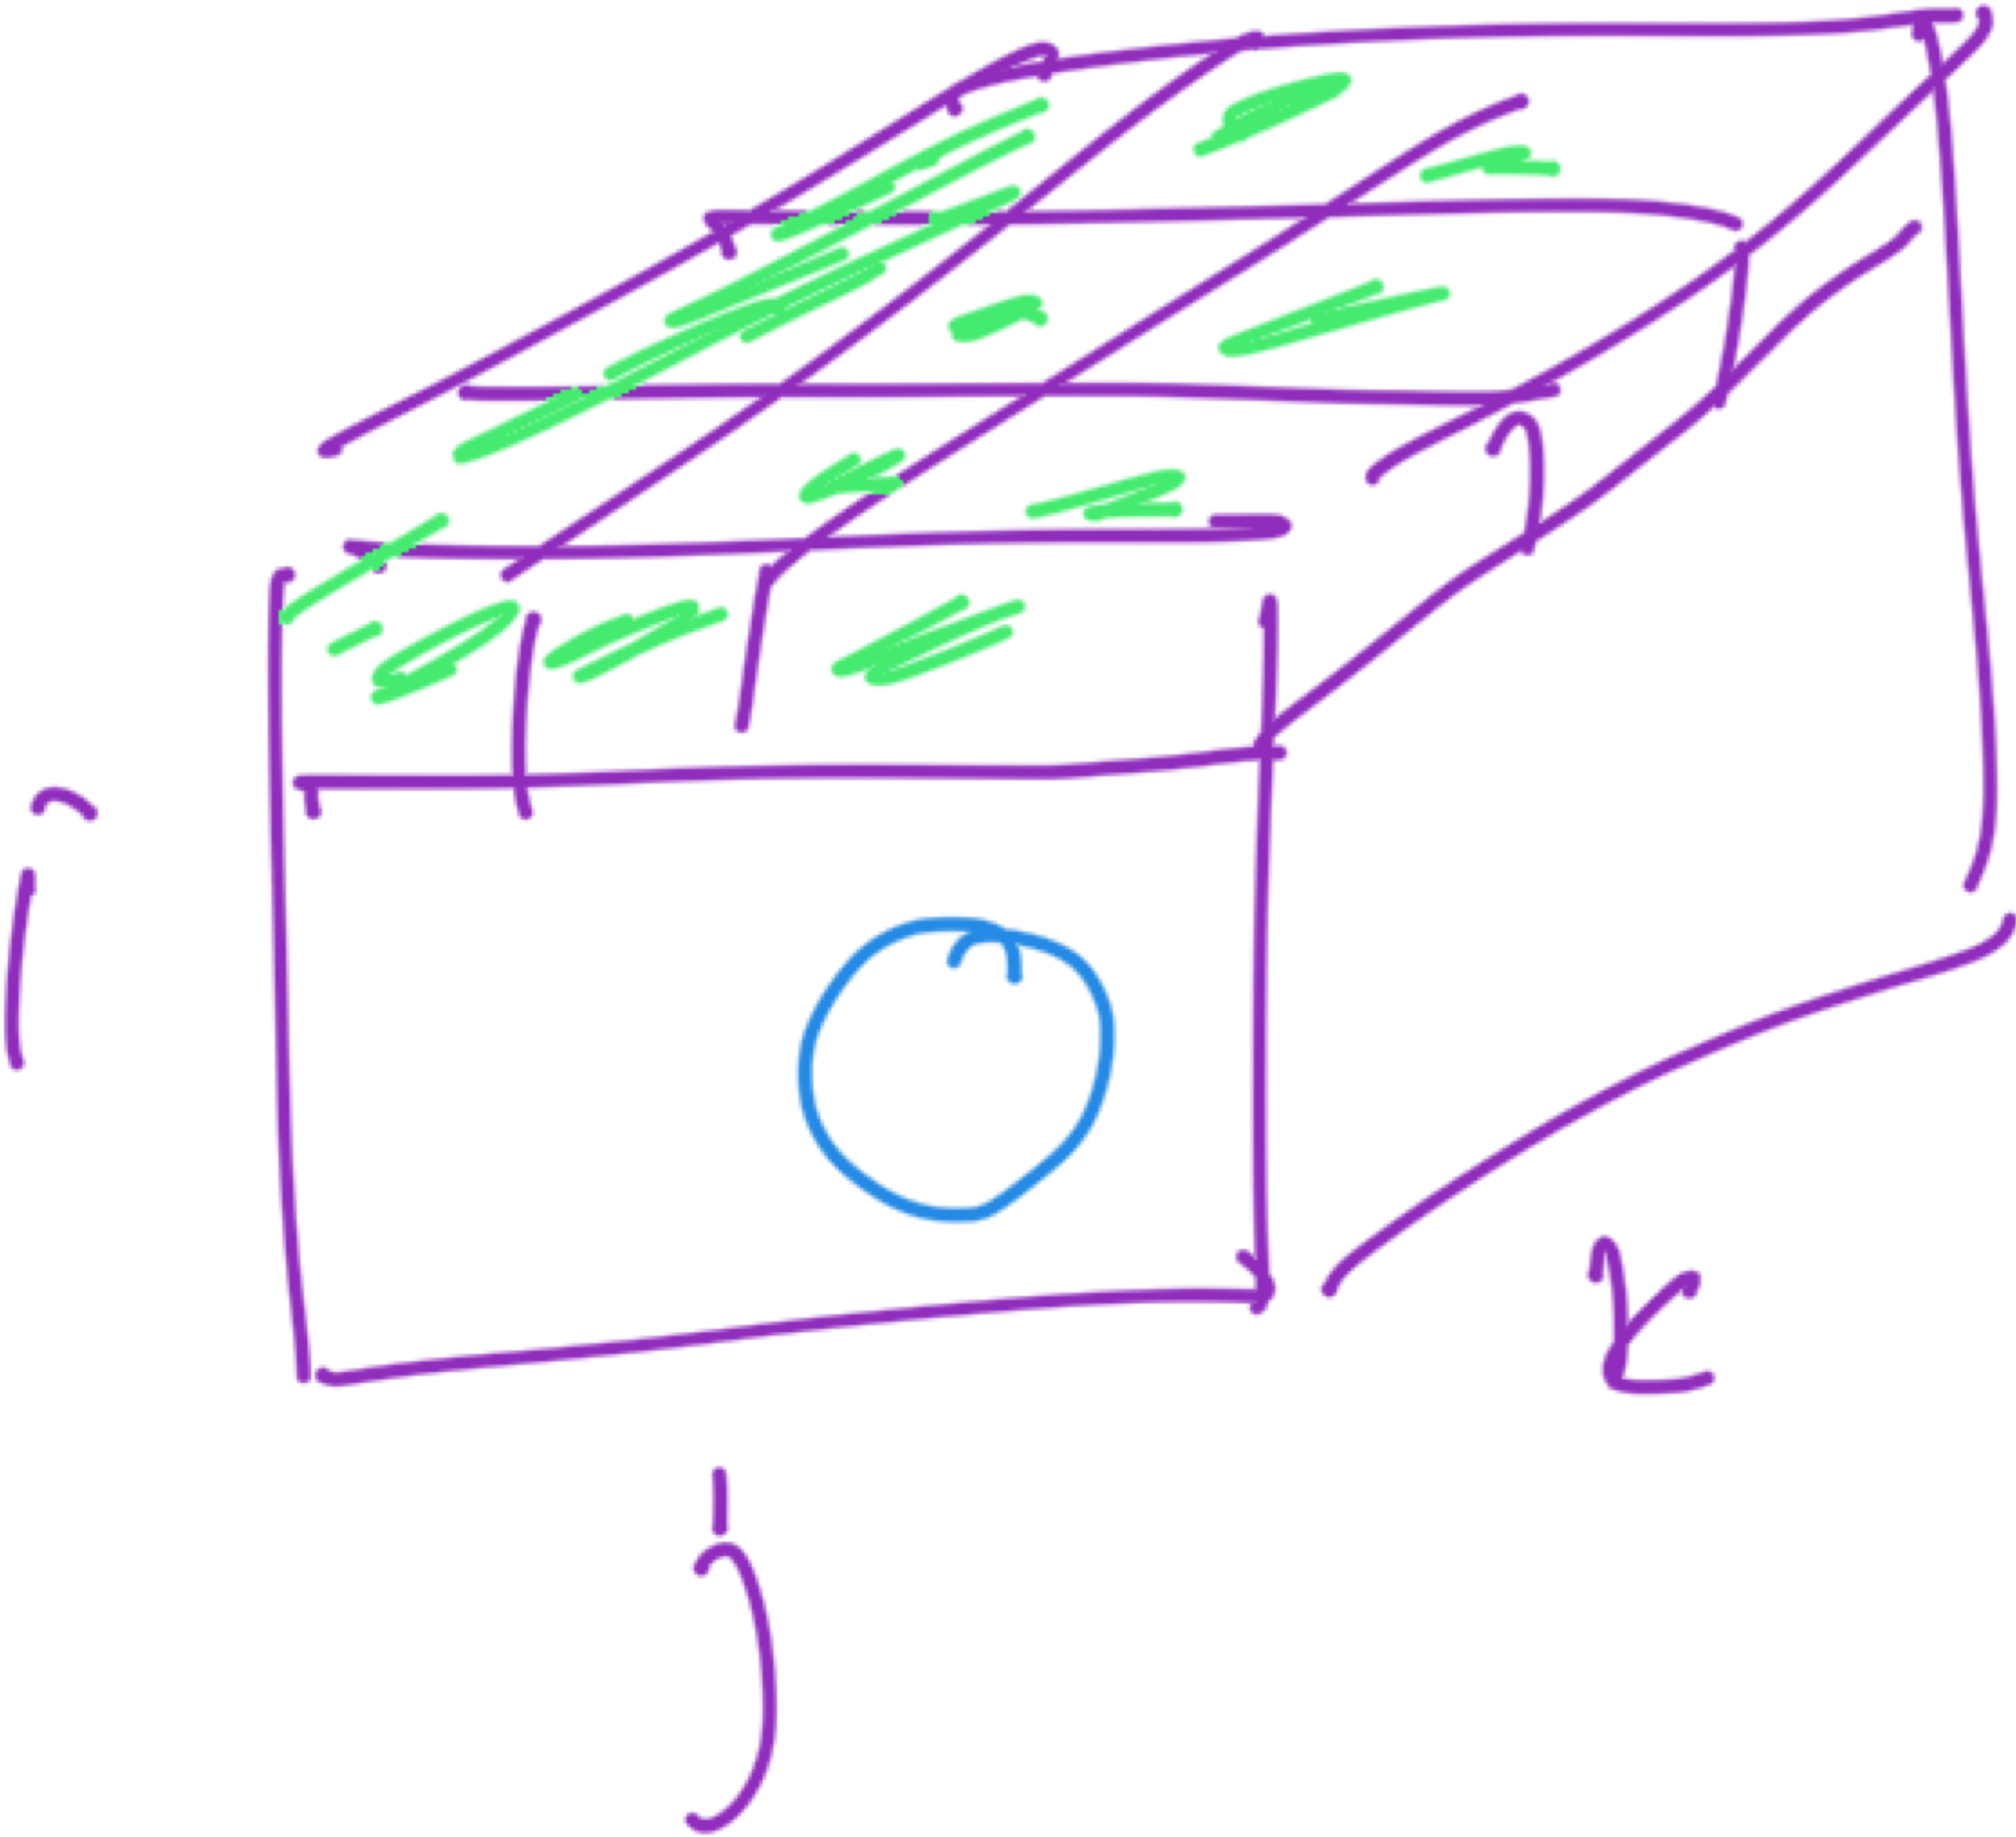
\includegraphics[scale=0.05]{smallBox.PNG}

That the adjacent minors vanish on tensors in the model variety is clear by construction, and their linear independence can be seen by recognizing that each has a unique last non-zero entry index. 

{\color{magenta}the rest here is open still.} 

Generalizing this, we obtain: 
\begin{proposition}
	Does the join variety $V_M$ have the expected dimension? Meaning we just add the dim of  hierarchical model from Hosten-Sullivant and $\prod d_i$? (minus 1.) 
\end{proposition}
\begin{proof}
	tbd.
\end{proof} 




\begin{thebibliography}{10}

\bibitem{AAC}
J.~Simonis and A.~Ashikhmin: {\em Almost affine codes},
Des.~Codes Cryptography, 14(2):179--197, 1998.

\bibitem{BenEfraim}
A.~Ben-Efraim: {\em Secret-sharing matroids need not be algebraic},
Discrete Math., 339(8):2136--2145, 2016.

\bibitem{DSS}
M.~Drton, B.~Sturmfels and S.~Sullivant: {\em Lectures on Algebraic Statistics}
Oberwolfach Seminars, Vol 40, Birkh\"auser, Basel, 2009.

\bibitem{FS86}
Ove Frank and David Strauss. Markov Graphs.� Journal of the American Statistical Association, vol. 81, no. 395, 1986, pp. 832--�842. JSTOR, https://doi.org/10.2307/2289017. 

\bibitem{M2}
D.~Grayson and M.~Stillman:
{\em Macaulay2, a software system for research in algebraic geometry},
available at \url{http://www.math.uiuc.edu/Macaulay2/}.

\bibitem{HoSu02}
S.~Ho\c{s}ten and S.~Sullivant: 
Gr\"obner Bases and Polyhedral Geometry of Reducible and Cyclic Models,
Journal of Combinatorial Theory, Series A,  100(2):277-301, 2002. 

\bibitem{Kir}
G.~Kirkup: {\em Random variables with completely independent subcollections},
Journal of Algebra {\bf 309} (2007) 427--454.

\bibitem{KayvanAleSteffen}
S.L. Lauritzen, A. Rinaldo, and K. Sadeghi:
On Exchangeability in Network Models (2019), 
Journal of Algebraic Statistics, 10 (1), 85--113

\bibitem{Mat92}
F.~Mat\'u\v{s}: {\em Ascending and descending conditional independence relations},
Transactions of the Eleventh Prague Conference on Information Theory, Statistical Decision Functions and Random Processes,
Vol.~B, pp.~189--200, Academia Prague.

\bibitem{Mat94}
F.~Mat\'u\v{s}: {\em Probabilitistic conditional independence structures and matroid
theory: background}, Int.~J.~General Systems {\bf 22} (1994) 185--196.

\bibitem{Mat99}
F.~Mat\'u\v{s}: {\em Matroid representations by partitions},
Discrete Math., 203(1-3):169--194, 1999.

\bibitem{MPSSW}
J.~Morton, L.~Pachter, A.~Shiu, B.~Sturmfels and O.~Wienand:
{\em Convex rank tests and semigraphoids},
SIAM Journal on Discrete Mathematics {\bf 23} (2009) 1117--1134.

\bibitem{Oxley}
J.~Oxley: {\em Matroid theory},
2nd ed., Oxford University Press, 2011.

\bibitem{KayvanAle}
K. Sadeghi and A. Rinaldo: Hierarchical Models for Independence Structures of Networks,  (2020), Statistica Neerlandica, 74, 439--457

\bibitem{Stu02}
B.~Sturmfels: {\em Solving Systems of Polynomial Equations},
Amer.~Math.~Soc., CBMS Regional Conferences Series, No 97, Providence, Rhode Island, 2002.

\bibitem{White}
N.~White, editor: {\em Theory of matroids}, volume~26.
Cambridge University Press, Cambridge, 1986.

\end{thebibliography}
\end{document}
